\documentclass[12pt]{article}
\usepackage{graphicx}
\usepackage{hyperref}
\usepackage{amsmath}
\usepackage{amssymb}
\usepackage[numbers, square, sort&compress]{natbib}
\title{Chapter 1: Introduction}
\begin{document}
\maketitle


Drug discovery is an arduous journey with many unknowns that may lead to failures. To perform many trials iteratively, computer simulations are convenient, enabling tens of thousands of calculations. This number of calculations can provide crucial insights and rule out dead ends early in the discovery cycle. Drug discovery is a multi-faceted science that requires art, innovative thinking, and often luck. For luck, we have no control; the best we can do is base our science on a solid foundation. In computational chemistry and biology, we often ask: how do we train computers to think like humans? This is not a concern because we do not need to train computers to think like humans. In fact, computers are extremely fast but dumb machines. In contrast, humans are extremely slow, lazy, yet smart thinkers. Now, the division of labour between humans and computers should be straightforward: let the computers handle the repetitive tasks of solving several complex mathematical equations that can be programmed to model chemistry and biology. This is done by employing the laws of physics that govern the movement of the atoms, and therefore molecules. Humans can focus on the complex decision-making steps that are beyond mathematical equations. However, with generative artificial intelligence (\textbf{GenAI}), computers can perform some level of thinking. However, their chemical and biological validity, in general, remains to be tested. GenAI, therefore, deserves appreciation for at least recognising the idea that computers could be made to think, not in a biological sense, but rather in a mathematical sense, which can be converted into chemical or biological models. However, the latter part has been extremely challenging and is yet to be fully conquered. 

This book ensures that the reader, perhaps a beginner, is aware of many assumptions that enable quick calculations. Also, thoroughly understand the limitations of these methods and use them to perform calculations for which they are meant or developed. Certain critical assumptions ensure the speed of the calculations by neglecting solvation effects or implicitly treating the entropy component of the free energy of binding. It is also not uncommon to neglect entropy to speed up calculations. These, and more limitations, will be discussed in great detail in the later chapters of this book. It must be noted that such assumptions are important to ensure that calculations are fast enough to complete several hundred or thousands of docking calculations per day, as required to virtually screen large databases comprising a few million to a billion molecules. 


This chapter can be viewed as a brief summary of the topics that will be covered in greater detail in the following chapters. Note that this book is intended to be a practical guide; therefore, we will emphasise the practical aspects of molecular docking that one needs to know before employing it to generate lead ideas or hit finding. We have made efforts to cover the theoretical foundations of topics we deem crucial to the successful application of molecular docking. Despite the effects, we do not claim this book to be a comprehensive text to cover all theoretical foundations of molecular docking. We further encourage readers to start practising molecular docking, even if they think they know nothing about the topic. We claim, based on our personal experience learning several computational tools, that most learning happens by trying first and then consulting books like this one to sharpen your understanding. 



\section{Molecular Recognition and Binding}

Understanding protein-ligand interactions at the atomic or molecular level is central to studying how small molecules interact with their biological receptor(s). Thus, the binding phenomenon may involve, but is not limited to, multiple types of non-covalent interactions such as hydrogen bonds, electrostatic interactions, van der Waals forces, and hydrophobic interactions. The binding affinity between a ligand and its receptor can be determined by the sum of favourable and unfavourable interactions, with the overall binding affinity dictating the strength of the complex. Protein-ligand binding affinity prediction quantifies binding strength, providing crucial insights for lead optimisation by altering functional groups to achieve maximum gains\cite {CH1_13}. 



The binding affinity is determined experimentally in the form of inhibition constants (K$_\text{i}$), dissociation constants (K$_\text{d}$), or half-maximal inhibitory concentrations (IC$_\text{50}$). If one is using isothermal calorimetry, then direct measurements of thermodynamic quantities like the change in enthalpy due to ligand binding ({$\Delta$}H), and the change in entropy (T{$\Delta$}S) can be made. However, experimental methods are expensive and time-consuming; thus, efficient computational methods capable of accurately predicting protein-ligand binding affinity are cost- and time-saving. Such accurate, high-quality computational methods can reduce the number of expensive experiments by filtering out unwanted molecules. The downside of computational methods is that they are heavily dependent on the empirical parameters used to make computing tractable.



\section{Historical Background}



\subsection{Early Foundations}

The conceptual foundations of structure-based drug design can be traced back to the early 20$^{\text{th}}$ century with Emil Fischer’s lock-and-key theory proposed in the late 1800s\cite{CH1_1}. This theory postulated that ligands fit into receptors like a key into a lock, representing the first mechanistic understanding of molecular recognition. This concept was later refined by Daniel Koshland’s induced-fit theory in 1958\cite{CH1_2}, which recognised that proteins are dynamic in nature and undergo conformational changes upon ligand binding. The induced-fit theory suggests that the protein's binding site is continually reshaped by interactions with ligands, providing a more accurate description of binding events than the rigid treatment.



\subsection{The Birth of the Protein Data Bank}

A pivotal moment in the history of SBDD occurred in 1971 with the establishment of the Protein Data Bank (PDB) as the first open-access, digital data resource in biology\cite{CH1_3}. The PDB was created to bring structural biologists onto a single platform and has evolved from a collaborative network to a full-fledged database with an extensive list of protein, nucleic acid-containing, and computational structures. The availability of three-dimensional atomic-level structures of biomacromolecules, determined by X-ray crystallography, nuclear magnetic resonance (NMR) spectroscopy, and electron microscopy, fundamentally transformed drug discovery.



\subsection{Structural biology Revolution}

Structural biology has undergone tremendous advances over the past few decades, with direct impacts on structure-based drug design (SBDD) \cite{CH1_4}.  X‑ray crystallography provided the first atomic‑resolution views of protein–ligand complexes and established the modern SBDD. High‑resolution crystal structures give crucial information on binding pockets, hydrogen‑bond networks, and water-mediated contacts. This information improves our understanding of drug-receptor interactions at the atomic level. Over time, improvements in crystallisation methods, synchrotron sources, and detectors increased throughput and resolution, making co‑crystal structures a routine decision‑making tool in medicinal chemistry. Furthermore, NMR spectroscopy extended this static picture of proteins by resolving their structures in solution under near‑physiological conditions\cite{CH1_4}. 

The most recent advancement has been in cryogenic electron microscopy (Cryo-EM). Improvements in direct electron detectors, image processing algorithms, and microscope stability have enabled near atomic-level resolution for large complexes and membrane proteins that were previously intractable to crystallography or NMR. Single particle cryo‑EM routinely yields structures of GPCR–G protein complexes, ion channels, transporters, and multi‑subunit assemblies in multiple functional states, providing unprecedented insights into conformational landscapes and ligand‑induced transitions. This has transformed SBDD for membrane proteins: structures of clinically important targets such as Transient Receptor Potential (TRP) channels,  Cystic Fibrosis Transmembrane Conductance Regulator (CFTR), and GABA receptors have revealed binding sites, gating mechanisms, and off‑target liability determinants that now guide design of safer and more selective small molecules\cite{CH1_5}.



\subsection{Evolution of molecular docking methods}

Molecular docking has evolved from a geometric-fitting algorithm for rigid receptors and ligands to algorithms that can handle flexibility in both ligands and receptors simultaneously. The first widely recognised docking approach was developed by Kuntz and co-workers in 1982 and implemented in the program DOCK.\cite{CH1_6} This method treated both receptor and ligand as rigid bodies, and emphasised geometric complementarity: ligands were positioned in binding sites by matching molecular shape using spheres and surface representations. This “first-generation method” established the conceptual framework for pose prediction and ranking; however, it neglected conformational flexibility and detailed energetics due to computational limitations.

In the 1990s and early 2000s, many groups followed with major improvements to increase the accuracy of the docking method. Search algorithms such as systematic, Monte Carlo-based, and genetic algorithms were employed to enhance ligand sampling and identify the bioactive conformation. Since docking accuracy also depends on scoring functions, empirical and force field-based scoring functions were developed to approximate binding affinity.\cite{CH1_7, CH1_8} Programs such as AutoDock incorporated a Lamarckian genetic algorithm and grid‑based energy evaluation, which allowed a routine docking of ligands with many rotatable bonds against rigid receptors.\cite{CH1_9} As the speed of docking ligands increased, this allowed for docking-based virtual screening of large chemical databases for hit identification, which significantly improved the productivity of early phase drug discovery. 



The next logical improvement focused on adding receptor flexibility to account for the induced-fit effect to mimic the physiological binding phenomenon. However, the additional degree of freedom came at the cost of computational speed\cite{CH1_8}. This was partially remedied by ensemble docking, which means that, instead of docking with full receptor flexibility, docking was performed across several protein conformations that might have been reported experimentally or generated from short runs of molecular dynamics simulations. 

Another milestone in the development of molecular docking methods was the ability to address covalent docking. Several of the drugs in the oncology section show their anticancer properties by covalently binding to their target. This was possible with algorithms capable of sampling non-covalent pre-reactive ligand topologies, followed by refining poses using post-reactive topologies that include the covalent bond\cite{CH1_11,CH1_12}.



Recent developments have focused on leveraging machine learning–based scoring functions, the explicit treatment of structural water, and dynamic docking approaches that couple molecular dynamics with docking searches\cite{CH1_10}. Taken together, these improvements over several decades have significantly improved both computational speed and accuracy. Nowadays, screening a large library of millions to billions of molecules is tractable. This can be attributed equally to parallel improvements in docking algorithms and to the computing power of modern computers and supercomputers.



\section{Structure-based drug design}

Structure-based drug design (SBDD) uses knowledge of receptor structure and its binding site to understand ligand shape and the interactions required for binding. The lock-and-key hypothesis is the main assumption underlying the development of software tools for SBDD. Therefore, the quality of the results depends on two things, assuming the software used is accurate (more on this in later chapters explaining why this is not always true):

\begin{itemize}

    \item Quality of the receptor structure

    \item Confidence with which the binding site information is known

\end{itemize}

The objective of molecular docking is to predict the binding modes and, thus, the affinities of small molecules to their target receptors. It models the interaction between the atoms of a small molecule and the receptor. Generally speaking, molecular docking is possible between any two (or more) chemical or biological entities, such as protein-protein, protein-DNA, protein-RNA, and all such combinations observed in biology. All aforementioned binding and recognition follow the same rules of interaction as those governed by the laws of physics. However, computationally, different potential energy functions are needed to model these bindings. We mainly focus on small-molecule protein docking; however, these discussions should apply to other types of docking. 



\subsection{Principles of Structure-Based Drug Design}

Structure-based drug design is fundamentally dependent on knowledge of the biological target's three-dimensional structure. The iterative process of SBDD begins with selecting a potential target, followed by ligand identification. The target may be a macromolecular protein involved in biosynthetic pathways. The three-dimensional structure of the protein is resolved using sophisticated techniques, including X-ray crystallography, nuclear magnetic resonance spectroscopy, and cryo-electron microscopy. Once the structure of the target is identified, it is necessary to investigate the properties of the protein, such as the presence of cavities, clefts, amino acid sequences, and allosteric pockets. Using various available algorithms, drug-like molecules from large databases of small molecules or compound fragments can be docked into the binding cavities of the target protein.



\subsection{The SBDD Workflow}

\textbf{Figure \ref{fig:sbdd_workflow}} shows a typical workflow for computational drug discovery. Depending on the chemical and biological information available, one might proceed with a structure-based or ligand-based approach. 

\begin{figure}[hbt!]

    \centering

    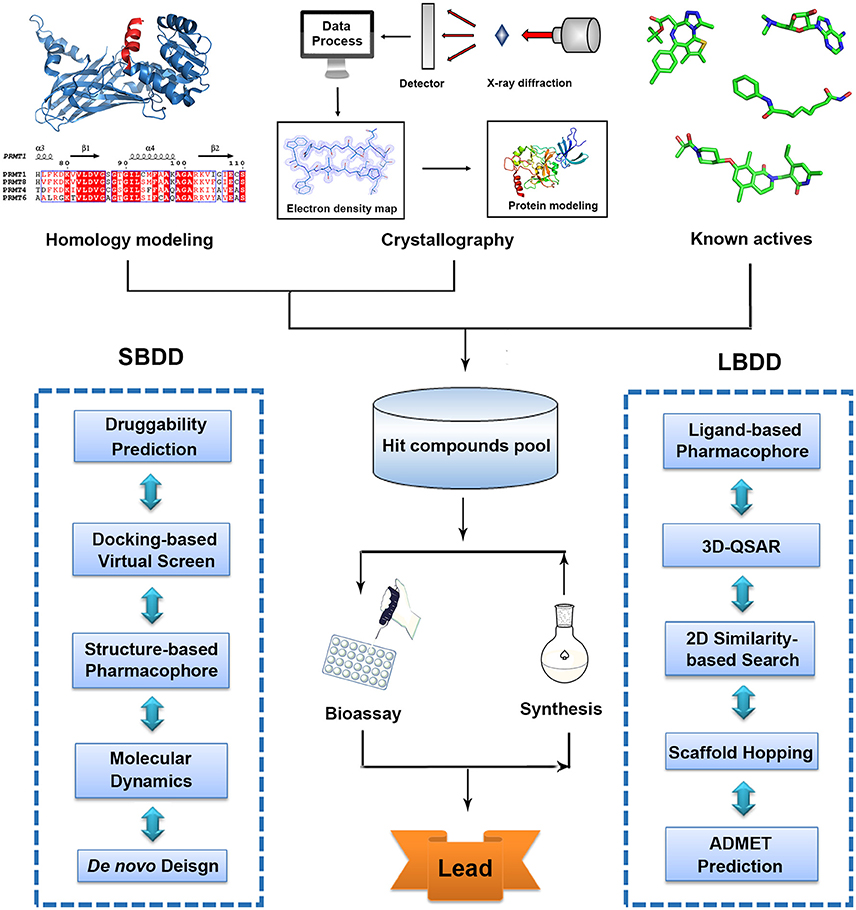
\includegraphics[width=1\textwidth]{../Figs/SBDD.jpg}

    \caption{A typical computational workflow for drug design. This figure also compares an alternative workflow, ligand-based drug design (LBDD), which is used when receptor information is unavailable. This image is reproduced from\cite{CH1_14} under the Creative Commons Attribution License (CC BY) licence.} 

    \label{fig:sbdd_workflow}

\end{figure}



\subsubsection{Druggability and Target Selection}

Druggability refers to the likelihood that a small molecule or any biological entity can modulate a biological target. The first step in SBDD is choosing an appropriate target, followed by evaluating its structure. Targets must possess characteristics that make them amenable to small molecule binding, including accessible binding sites with suitable geometry and chemical properties.



\subsection{Binding Site Identification}

Knowing the location of the binding site before docking processes significantly increases docking efficiency. In many cases, the binding site is known before docking ligands into it, and information about the site can be obtained by comparing the target protein with a family of proteins sharing a similar function or with proteins co-crystallised with other ligands. In the absence of knowledge of the binding sites, cavity detection programs or online servers such as GRID\cite{CH1_16}, SurfNet\cite{CH1_16}, and many others can be utilised to identify putative active sites within proteins. Docking without any assumption about the binding site is called blind docking. This could also be a strategy to explore potential sites that may bind cavities not previously identified. 



\subsubsection{Determination and Preparation of receptor}

The SBDD workflow begins with obtaining the target receptor's three-dimensional structure. Structures can be obtained from the Protein Data Bank, which currently holds over 251,217 (\textit{as of March 2026}) atomic-level 3D structures of biomolecules. When experimental structures are not available, protein modelling, including homology modelling and \textit{ab initio} techniques, allows for predicting the three-dimensional structure. Selection of an appropriate receptor structure from the PDB is a critical step, as multiple crystal structures are often available for the same receptor. A systematic approach to selecting the appropriate receptor structure must consider factors such as resolution, completeness, ligand presence, and biologically relevant conformations. Recent advances include AlphaFold\cite{CH1_15}, which has revolutionised life sciences by predicting over 200 million protein structures available in the AlphaFold Database, far exceeding the number of experimentally resolved structures.



\subsubsection{Ligand Library Preparation}

After target structure preparation, the next step is to prepare compound libraries for virtual screening. Ligand preparation includes generating three-dimensional coordinates, assigning appropriate protonation states, and optimising geometries using suitable force field parameters. Compound libraries can range from commercially available compounds to virtual libraries representing synthesisable chemical space.



\subsubsection{Virtual Screening}

Virtual screening is a computational technique used to search large libraries of compounds and identify those most likely to bind to a drug target. Structure-based virtual screening uses molecular docking to test large libraries of compounds for potential binding to target proteins. The virtual screening process typically involves multiple stages of filtering and refinement. Initial rapid screening of large compound collections with fast scoring methods is followed by more detailed analysis of top-ranked compounds with more sophisticated scoring methods. Consensus virtual screening between multiple docking programs can increase the reliability of results. Top-scoring molecules from virtual screening with high affinity toward the target protein are synthesised and tested in \textit{in vitro} biochemical assays. Ligands with desired therapeutic activities are further evaluated for efficacy, affinity, and potency studies. Structural insights into the complex of ligand-protein assist the analysis of a variety of binding conformations and interactions.





\section{Molecular Docking: Concepts and Methods}

In this introductory chapter, we cover, albeit as a brief note, all topics that will be covered in great detail in subsequent chapters.



\subsection{Fundamentals of Molecular Docking}

Molecular docking is a computational technique that predicts the binding affinity of ligands to receptor proteins. The docking process involves two basic steps: prediction of the ligand conformation (referred to as the pose) and its position and orientation within the binding site, and assessment of the binding affinity. These two steps are related to sampling methods and scoring functions, respectively. The scoring function guides and determines the most plausible poses from thousands of possible poses. It can be used to determine the binding mode and site of a ligand, predict binding affinity, and identify potential drug leads for a given protein target. Despite intensive research over the years, accurately and rapidly predicting protein-ligand interactions remains a challenge in molecular docking.



\subsection{Rigid vs Flexible Docking}

The treatment of molecular flexibility represents a fundamental consideration in docking methodology. Early docking methods treated both the ligand and the receptor as rigid bodies, based on the lock-and-key theory. Docking with a flexible ligand and a rigid receptor has been performed for a long time and remains the most popular method. This approach balances computational efficiency with reasonable accuracy for many applications. Given the limitations of computer resources, flexible ligand docking with rigid receptors has dominated the field, though recently many efforts have been made to address receptor flexibility. Flexible receptor docking, especially backbone flexibility, remains a major challenge for current docking methods. The induced-fit theory suggests that ligand and receptor should be treated as flexible during docking, as this approach can better describe binding events than rigid treatment\cite{CH1_18}.



\subsection{Docking Algorithms}

Multiple algorithmic approaches have been developed for conformational sampling in molecular docking. Common search algorithms include genetic algorithms, Monte Carlo methods, simulated annealing, and systematic search approaches. The Lamarckian Genetic Algorithm implemented in AutoDock4\cite{CH1_9} successfully models flexible ligand binding, particularly useful for complex systems that require in-depth torsional and conformational exploration. AutoDock Vina\cite{CH1_19} introduced a multithreaded architecture that outperformed AutoDock4 by up to 100 times in docking throughput. On select benchmark datasets, Vina correctly placed native-like poses in the top three results in more than 93\% of situations, particularly excelling in polar and charged receptor settings. The Attracting Cavities algorithm represents another important approach, positioning cloud points in protein cavities and using these as guides for ligand placement and optimisation.





\subsection{Scoring Functions}


Scoring functions are mathematical functions\cite{CH1_20} used to approximately predict the binding affinity between two molecules following molecular docking. During docking, the search algorithm explores a vast number of conformations for each molecule, and scoring functions evaluate the quality of these docking poses, guiding the search toward relevant ligand conformations.

The scoring function calculates a score or an estimate of the binding affinity of a particular pose. This represents the thermodynamics of the protein-ligand interaction to distinguish true binding modes from all others explored and rank them accordingly. Scoring functions must accomplish three primary tasks:
\begin{itemize}
\item The first is to distinguish experimentally observed binding modes by associating them with the lowest binding energies in the energy landscape, relative to all other poses (pose prediction). 
\item The second is to classify active and inactive compounds during virtual screening. 
\item And the third is predicting binding affinity, ranking compounds correctly by potency (binding affinity prediction), which is the most challenging task. 
\end{itemize}
An ideal scoring function would be able to perform all three tasks effectively; however, given several limitations of current scoring functions, they exhibit different accuracies across distinct tasks due to modelling assumptions and simplifications made during their development. 

\section{Current challenges and limitations of molecular docking}

\subsection{Limited accuracy}

Despite considerable success, accurately and rapidly predicting protein-ligand interactions remains a challenge in molecular docking. One of the biggest challenges is modelling receptor flexibility to account for induced-fit behaviour fully. Most molecular docking tools provide high ligand flexibility, while the protein is kept more or less fixed or given limited flexibility to residues within or near the active site. Providing complete molecular flexibility to the protein exponentially increases the space and time complexity of computation. The scoring function's accuracy in estimating binding affinity is another fundamental limitation. Most current scoring functions are generic models derived from large-scale experimental data of ligand-target complexes. However, a universally accurate scoring function remains the greatest challenge. Scoring functions must balance speed with accuracy, and the trade-offs inherent in this balance limit overall performance. The traditional approach to train empirical scoring functions using linear regression to optimise the correlation between predicted and experimental binding affinities does not yield functions with optimal docking capabilities\cite{CH1_21}.



\subsection{Computational Demands}

Virtual screening of large compound libraries requires substantial computational resources. While methods like AutoDock Vina, with its multithreaded architecture and GPU-accelerated variants, have dramatically improved throughput, screening millions of compounds remains computationally intensive. The balance between computational speed and accuracy remains a critical consideration in method development\cite{CH1_22, CH1_23}.



\subsection{Validation Requirements}

Computational predictions must ultimately be validated through experimental testing. The gap between computational predictions and experimental validation can be substantial, with many computationally predicted hits failing to show activity in biological assays. The reasons could be several-fold, including assumptions incorporated into scoring functions to improve computational speed. Many scoring functions entirely ignore the entropy component of binding, which is a significant penalty component of binding free energy ($\Delta$G).



\subsection{Solvation Effects}

Solvation effects remain a major bottleneck in molecular docking and scoring because they couple tightly to both enthalpic and entropic components of binding, yet must be approximated for enhanced throughput.  Most docking scoring functions treat the solvent implicitly or via empirical terms, which can reproduce experimental solvation energies in isolation but often fail to improve, and sometimes even worsen.  As a result, the incomplete and approximate treatment of solvation is recognised as one of the principal reasons why current docking scores show limited quantitative reliability for affinity prediction, even when sampling is adequate\cite{CH1_24}.



\section{Upcoming improvments}

\subsection{Artificial Intelligence and Machine Learning}

The integration of artificial intelligence and machine learning with structure-based drug design represents one of the most promising future directions. AI can transform drug discovery and early drug development by addressing inefficiencies in traditional methods. Machine learning-based scoring functions are showing promise for outperforming traditional approaches while displaying greater generalizability.

Geometric deep learning, an emerging neural network-based machine learning approach, has been applied to macromolecular structures, with particular relevance for structure-based drug discovery. Applications include molecular property prediction, ligand binding site and pose prediction, and structure-based de novo molecular design. Deep learning models can leverage interatomic potentials between complexes’ bound and unbound states for robust predictions.



\subsection{Quantum Computing}

The upcoming power of quantum computing promises to enhance molecular dynamics simulations and drug discovery capabilities. Quantum computing could address some of the computational limitations that currently constrain full molecular flexibility treatment and extensive conformational sampling. The powerful synergy of AI, machine learning-enhanced molecular dynamics simulations, and quantum computing will aid in developing innovative therapeutic strategies.





\section{Summary}

Structure-based drug design has fundamentally transformed pharmaceutical research, evolving from theoretical concepts to essential tools in modern drug discovery. The field has delivered remarkable successes, from HIV protease inhibitors to recent breakthroughs in targeting previously undruggable proteins like KRAS. The Protein Data Bank’s contribution to facilitating the discovery has been significant towards new drugs approved by the FDA underscores the profound impact of structural information on therapeutic development. Despite significant advances, challenges remain in achieving universal accuracy in binding affinity prediction, handling protein flexibility, and developing scoring functions that perform optimally across diverse target classes. The integration of artificial intelligence, machine learning, and revolutionary structure-prediction methods such as AlphaFold promises to address many current limitations and open new frontiers in drug discovery. The future of SBDD will likely see greater integration of multiple computational approaches, including molecular docking and dynamics simulations, as well as machine learning and quantum computing. As computational methods become more sophisticated and experimental structural data continues to accumulate, structure-based drug design will play an increasingly central role in discovering safe and effective therapeutics. For beginners entering this field, the foundations presented in this book provide a medium to explore this area in depth, understand the subtle nuances, and make informed choices about the tools available. 



\bibliographystyle{unsrtnat}

\bibliography{chapter1}

\end{document}